\section{Introduction}
\label{sec:MAMT:intro}

With the rapid advances in sensor design, data storage and networking, we are facing an explosive growth of complexity in analyzing failure (or event) in multivariate time series data. Failure analytics system can be identified from the knowledge data discovery process where the output gives the fault signatures that relate to the failure, while the input data correspond to recorded sensor measurements that are considered as features. These high-frequent, large-scale data often require fleet level analysis, which not only involve the event assets, but also the healthy assets (usually much more than those event ones), therefore a unique fault signature relates to the failure can be found and a detector with low-false-alarm-rate can be created. The output of such signature should consist of or directly relate to the weighting of input sensor, therefore more effectively support the root cause analysis. Furthermore, a forecast model can be built consequently that gives early warning of the same failure in the future.      


Besides large-volume of data on the fleet level, we are also facing the following challenges in finding such signatures: 
1) The fault signatures usually exist in multivariate time series involving a lot of assets, which makes it hard to detect by any univariate and uni-asset analytics;
2) While the event time can be known, the time that faulty signatures happen is usually unknown, and could be different from case to case, which makes it difficult to detect by any (semi-)supervised machine learning techniques. 

Figure~\ref{fig:MAMT:motivation} shows the two signature examples from ground truth by domain experts. In Figure~\ref{fig:MAMT:motivation:01} the signature appears $15$ days before the failure, and the signature is with small value on feature A and large value on feature B. While in Figure~\ref{fig:MAMT:motivation:02} the signature appears almost one month before the failure, where there is a level-shift on feature C that can be depicted by auto-correlation (auc). It is interesting and important to notice that 1) both of these examples show significant lag between signature and failure, and 2) the lasting time of signature are different which is also unknown for the analytics. As a matter of fact, this ``lag" patterns are usual and could be with different reasons. One of the reasons is that the input sensors could be indirectly related to the failure. For example, an engine stall event may happen because some component is crack. But due to the complexity of the engine design, it takes certain time for such fault propagate to the whole system which leads to the final failure. Right before the crack, the vibration sensors of the faulty component can show strong vibrating patterns, which can be viewed as the faulty signature. But once the crack happen, this component becomes unconnected to the whole system and the vibration sensor recording become stable. Therefore the signature cannot be found right before the final failure but only before the time of crack.  

\begin{figure}[htb]
\centering
\subfigure[Event 1]{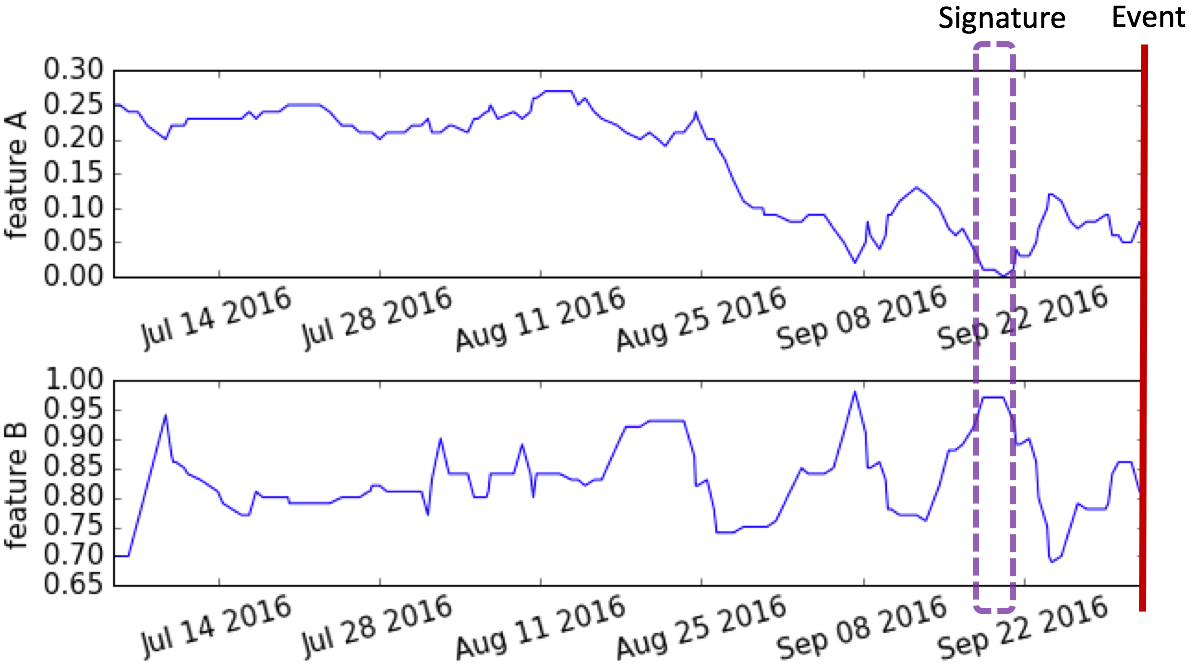
\includegraphics[width=3.1in]{pics/Motivation_1} \label{fig:MAMT:motivation:01}}
\subfigure[Event 2]{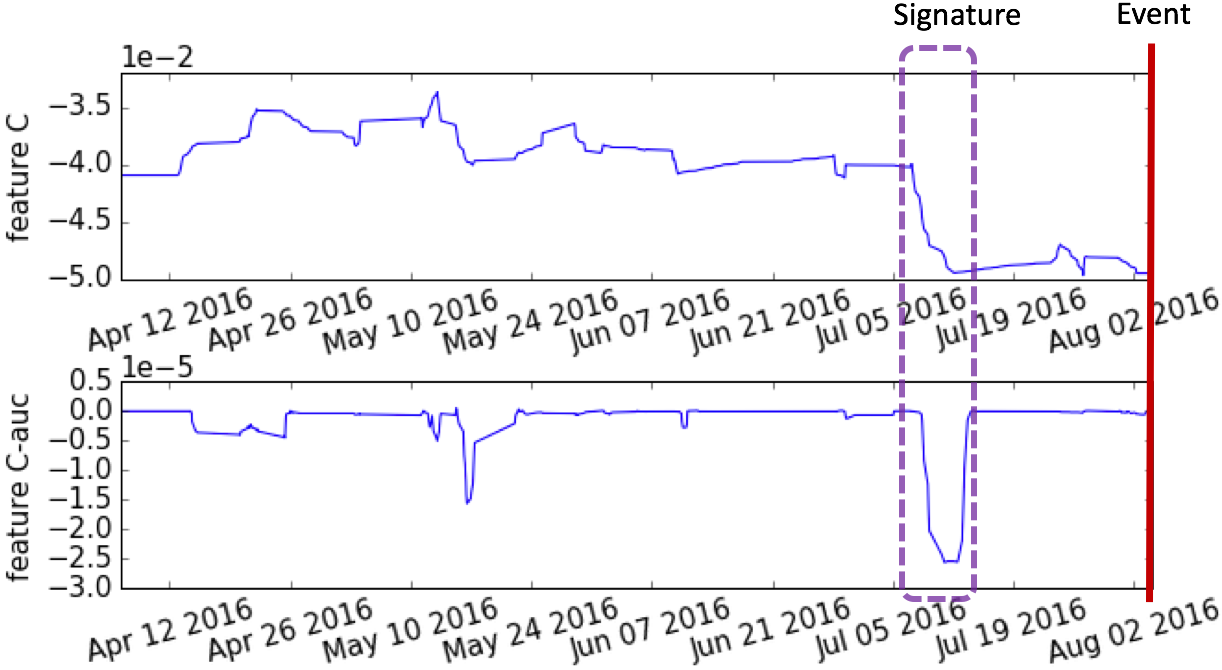
\includegraphics[width=3.1in]{pics/Motivation_2} \label{fig:MAMT:motivation:02}}
\caption{Two examples of fault signatures with lag to final failures (events). In Figure~\ref{fig:MAMT:motivation:01} the signature appears $15$ days before the failure, with small value on feature A and large value on feature B. While in Figure~\ref{fig:MAMT:motivation:02} the signature appears almost one month before the failure, where there is a level-shift on feature C that can be capture by auto-correlation (auc).}
\label{fig:MAMT:motivation}
\end{figure}

\begin{figure*}[tb]
\centering
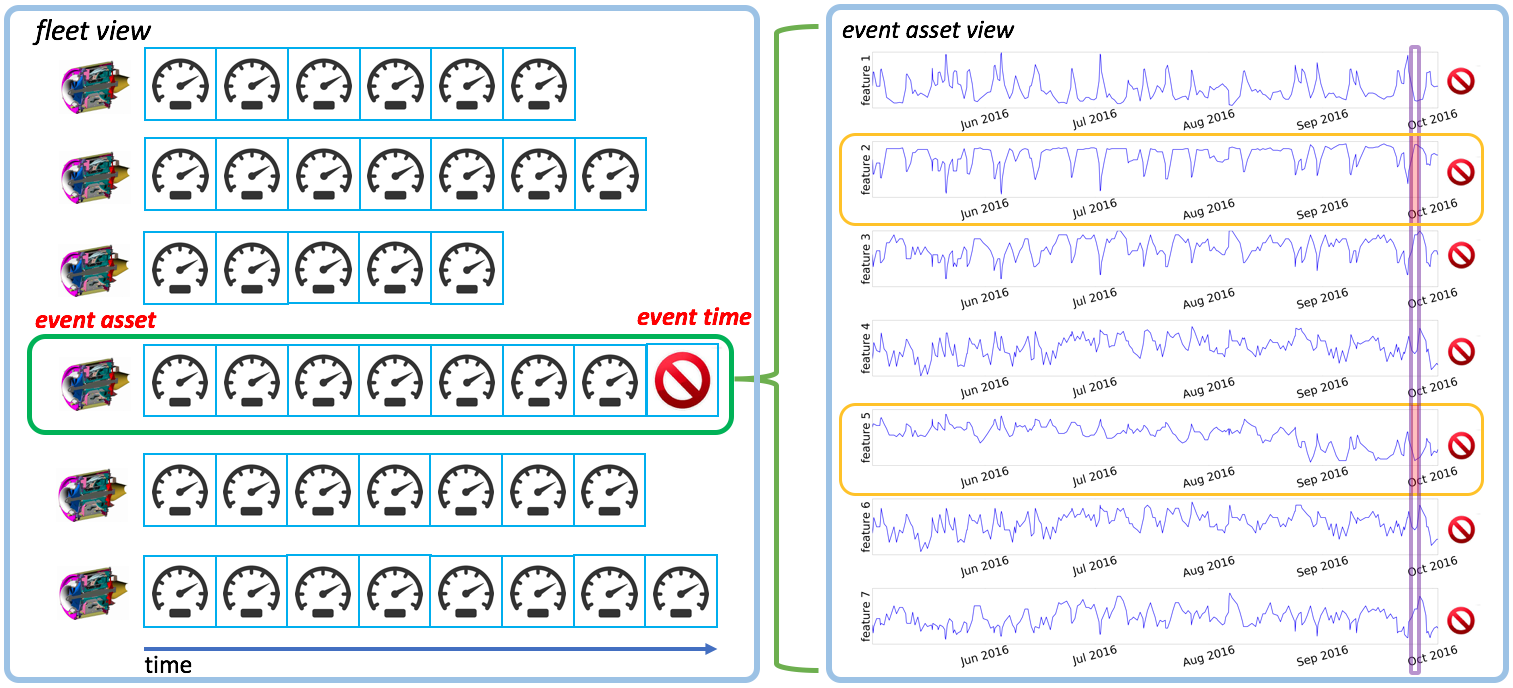
\includegraphics[width=5in]{pics/multi-view_structure}
\caption{Illustration of Multi-view Failure Analysis on Multivariate Time-series Data. Given the event asset and event time on the fleet level data, our model can provide the fault signature (marked by red shadow) on the feature level (rounded by yellow box) and timestamp level (rounded by purple box). }
\label{fig:MAMT:structure}
\end{figure*}

It can be easily imagined that, if we natively label the samples right before failure as ``1" and perform classic supervised machine learning algorithm \footnote{In a classic supervised setting, the event samples are considered as positive and usually labeled as ``1", while the other are considered as normal and labeled as ``0".}, we are not able to find such fault signature. The key difference of the problem, compared to the popular definition of supervised problems, is that \textbf{our label ``1"s are uncertain and even most of them could be wrong}. For example in Figure~\ref{fig:MAMT:motivation:01}, without any prior knowledge if we label all samples $30$ days before the final failure as ``1", the classic feature selection like random forest, lasso-based or mutual-information based methods will be easily failed, since only $10\%$ of ``1" are correct and the rest should be treated as $0$ (normal class). To handle this kind of problem, this paper proposes a Multi-view Failure Analysis on 
Multivariate Time-series Data (MAMT) which overcomes the limitations of classic supervised algorithms on such problem.  Our contributions are as follows:
\begin{enumerate}[(1)]
\item We proposed a novel fleet analytics model that aims to select key features that relate to the failure on multivariate time-series data, which can effectively support the root cause analysis.
\item Our proposed model, compared with the existing supervised methods, automatically detect the time of signature by filtering the ``wrong labels". 
\item Our proposed model, compared with the existing methods,
    achieves a similar or even lower time and space computational complexity, but a more desired effectiveness.
\end{enumerate}



Figure~\ref{fig:MAMT:structure} illustrates that such multi-view analytics is unique and different from the existing works on any supervised feature selection or instance selection for multivariate temporal data. The left side shows the data on the fleet-level view and the event asset and event time is already known. The right side shows the multivariate time series for the event asset, and the fault signature on the feature level (rounded by yellow box) and timestamp level (rounded by purple box) are unknown. Without any more prior knowledge (other than the event asset and event time), our model can provide the fault signature (marked by red shadow) on multi-view level.   


%Capabilities of this algorithm: 
%Output corresponding classifier/detector to detect the targeted failure events on the fleet level.
%Automatically detect the most relevant feature patterns among all events that support root cause analytics. 
%Automatically adapt/detect different lead time for each event.   
